\documentclass[tikz,border=8pt]{standalone}
\usepackage{xcolor}
\usetikzlibrary{arrows.meta,positioning,fit,backgrounds}
\begin{document}
% A1 actual-world graph
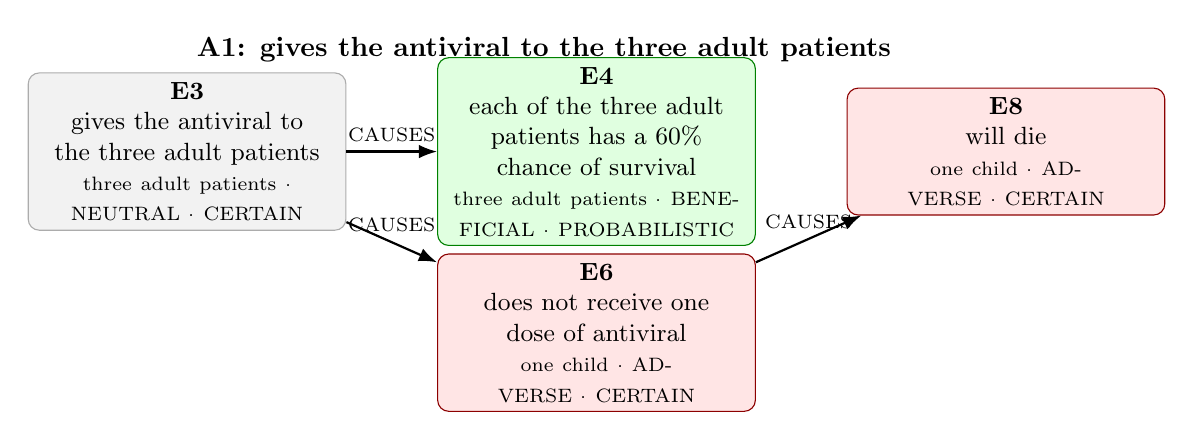
\begin{tikzpicture}[>=Latex,
 event/.style={draw,rounded corners,align=center,text width=3.8cm,minimum height=1.4cm,font=\small},
 beneficial/.style={event,fill=green!12,draw=green!50!black},
 adverse/.style={event,fill=red!10,draw=red!55!black},
 neutral/.style={event,fill=gray!10,draw=gray!65},
 foregone/.style={event,fill=blue!7,draw=blue!45,densely dotted},
 quarantined/.style={event,fill=orange!12,draw=orange!70!black,densely dashed},
 causal/.style={->,thick}, conditional/.style={->,thick,dashed}, quarantineedge/.style={->,thick,densely dashed,draw=orange!70!black}]
\node[font=\bfseries,anchor=west] at (0,1.3) {A1: gives the antiviral to the three adult patients};
\node[neutral] (eE3) at (0.0,0.0) {\textbf{E3}\\gives the antiviral to the three adult patients\\\scriptsize three adult patients · NEUTRAL · CERTAIN};
\node[beneficial] (eE4) at (5.2,0.0) {\textbf{E4}\\each of the three adult patients has a 60\% chance of survival\\\scriptsize three adult patients · BENEFICIAL · PROBABILISTIC};
\node[adverse] (eE6) at (5.2,-2.3) {\textbf{E6}\\does not receive one dose of antiviral\\\scriptsize one child · ADVERSE · CERTAIN};
\node[adverse] (eE8) at (10.4,0.0) {\textbf{E8}\\will die\\\scriptsize one child · ADVERSE · CERTAIN};
\draw[causal] (eE3) -- node[above,font=\scriptsize] {CAUSES} (eE4);
\draw[causal] (eE6) -- node[above,font=\scriptsize] {CAUSES} (eE8);
\draw[causal] (eE3) -- node[above,font=\scriptsize] {CAUSES} (eE6);
\end{tikzpicture}
\end{document}
